\documentclass[11pt,a4paper]{article}
\usepackage[margin=2.5cm]{geometry}
\usepackage{graphicx}
\usepackage{booktabs}
\usepackage{amsmath}
\usepackage{hyperref}
\usepackage{caption}
\usepackage{float}

\title{COMP0240 Coursework 1: Drone Structural Inspection\\Mission Planning Report}
\author{Bowen Zhu}
\date{March 2026}

\begin{document}
\maketitle

\section{Problem Statement}

This coursework addresses autonomous drone mission planning for structural inspection, where a drone must visit a set of viewpoints to photograph ArUco markers while avoiding obstacles. The challenge involves two sub-problems: (1) determining an efficient visitation order to minimise flight time and distance, and (2) planning collision-free paths through environments with varying obstacle densities. Four scenarios of increasing complexity test the system: Scenario~1 (10 viewpoints, 1 obstacle), Scenario~2 (10 viewpoints, 5 obstacles), Scenario~3 (20 viewpoints, 1 obstacle), and Scenario~4 (5 viewpoints, 10 obstacles). The baseline approach visits viewpoints in the order listed in the scenario file with no obstacle avoidance, serving as a performance reference.

\section{Methodology}

The optimised solution combines two algorithmic components: a Travelling Salesman Problem (TSP) solver for route optimisation and a 3D A* path planner for obstacle avoidance.

\subsection{Route Optimisation (TSP)}

The viewpoint visitation order is formulated as an open-loop TSP: starting from the drone's initial position, find the shortest tour visiting all viewpoints exactly once. The Euclidean distance between all pairs of viewpoints (including the start position) forms the cost matrix, with the return-to-start column set to zero since landing occurs at the final viewpoint.

For scenarios with $\leq$15 viewpoints (Scenarios~1, 2, and 4), exact dynamic programming solves the TSP optimally in $O(n^2 \cdot 2^n)$ time. For Scenario~3 (20 viewpoints), where exact methods become computationally prohibitive, simulated annealing provides a near-optimal heuristic solution. This hybrid approach balances optimality with computational feasibility.

\subsection{Obstacle Avoidance (3D A*)}

Before executing each segment, a collision check samples points along the straight-line path at 0.2m intervals. If any sample falls within an obstacle's bounding box (expanded by a 1.0m safety padding), the path planner activates.

The avoidance strategy uses a three-tier approach:
\begin{enumerate}
    \item \textbf{Elevation bypass}: Attempts to fly over obstacles by raising altitude incrementally (+2m, +3m, +4m, +5m above the higher endpoint), checking that the up, across, and down segments are all collision-free. This is the fastest strategy as it requires only 3 waypoints.
    \item \textbf{Full 3D A* search}: If elevation bypass fails, a grid-based A* search (resolution 0.5m, 26-connected neighbourhood) finds a path through 3D space. The resulting path is simplified by iteratively removing intermediate waypoints where direct line-of-sight exists.
    \item \textbf{High-altitude fallback}: As a last resort, the drone ascends to 9.0--9.5m altitude to fly above all obstacles.
\end{enumerate}

The yaw angle at each viewpoint is specified in radians in the scenario file and converted to degrees for the flight controller, ensuring the camera faces the correct direction for marker photography.

\section{Results}

\subsection{Optimised Performance}

Table~\ref{tab:results} summarises the optimised mission performance across all four scenarios, with baseline comparison where available.

\begin{table}[H]
\centering
\caption{Mission performance: baseline vs optimised.}
\label{tab:results}
\begin{tabular}{lcccccc}
\toprule
Scenario & Method & VP & Time (s) & Distance (m) & Avoidances & Success \\
\midrule
1 & Baseline  & 10/10 & 231.82 & 125.93 & 0 & 100\% \\
1 & Optimised & 10/10 & 126.37 & 59.00  & 1 & 100\% \\
\midrule
2 & Optimised & 10/10 & 143.23 & 59.00  & 1 & 100\% \\
\midrule
3 & Baseline  & 20/20 & 412.20 & 174.94 & 0 & 100\% \\
3 & Optimised & 20/20 & 213.50 & 81.18  & 1 & 100\% \\
\midrule
4 & Optimised & 5/5   & 112.95 & 47.78  & 3 & 100\% \\
\bottomrule
\end{tabular}
\end{table}

TSP optimisation achieves substantial improvements: 45.5\% time reduction and 53.1\% distance reduction for Scenario~1, and 48.2\% time reduction and 53.6\% distance reduction for Scenario~3. All scenarios achieve 100\% viewpoint visitation.

\subsection{Obstacle Avoidance Analysis}

Figure~\ref{fig:planned_actual} compares the TSP-planned straight-line paths against actual flight paths with A* obstacle avoidance. The distance overhead from avoidance varies with obstacle density:

\begin{itemize}
    \item \textbf{Scenarios 1--2} (1--5 obstacles): +6.1m overhead (+10.4\%), single elevation bypass each.
    \item \textbf{Scenario 3} (1 obstacle, 20 VP): +5.6m overhead (+6.9\%), minimal impact due to sparse obstacles.
    \item \textbf{Scenario 4} (10 obstacles): +17.4m overhead (+36.5\%), three elevation bypasses navigating through a dense obstacle field.
\end{itemize}

The elevation bypass strategy proved effective across all scenarios, avoiding the computational cost of full A* search while maintaining safe clearance. In Scenario~4, the drone ascended to z$\approx$5--7m to fly over obstacle clusters, with the longest avoidance segment (VP3$\to$VP4) spanning the full arena width.

\begin{figure}[H]
\centering
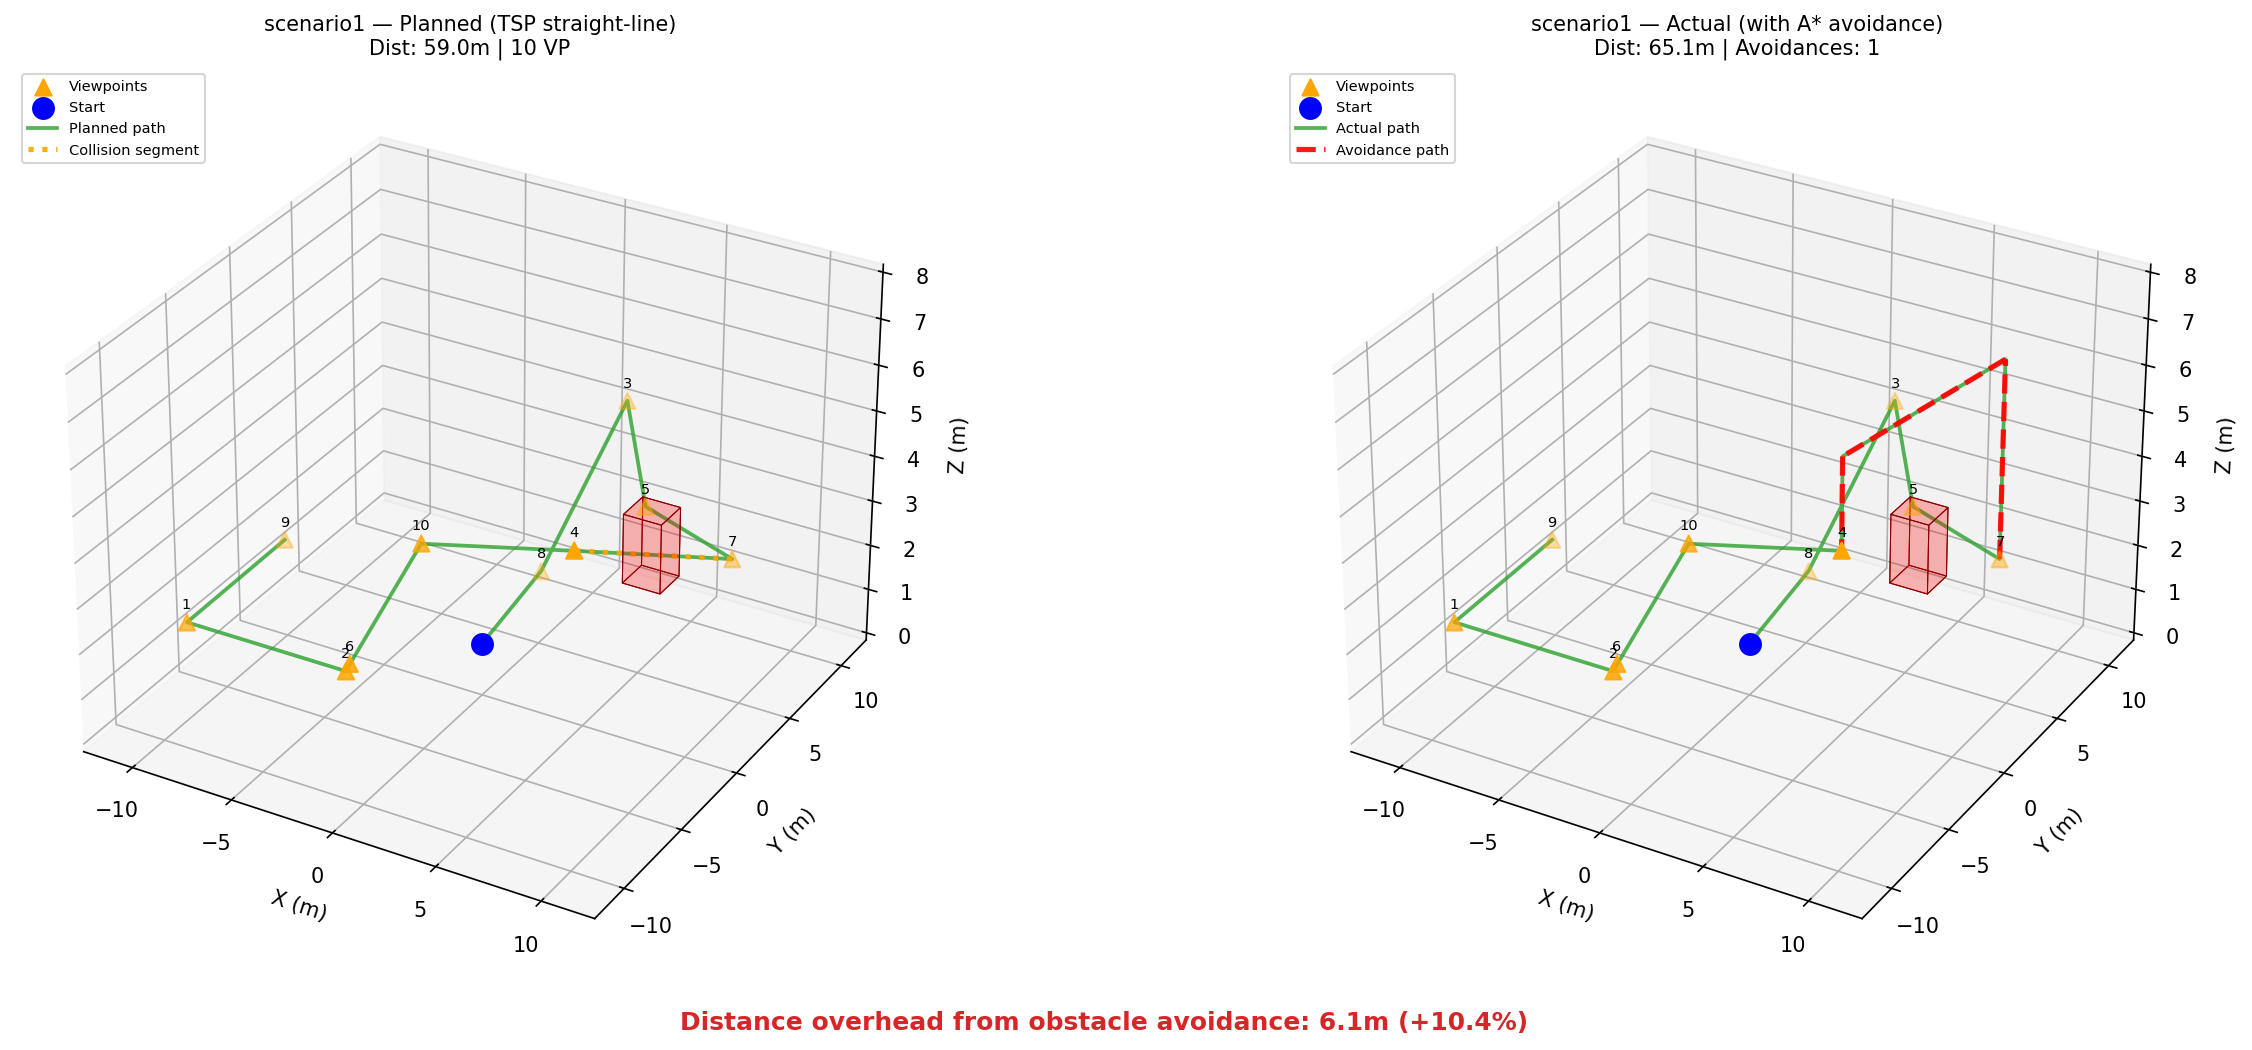
\includegraphics[width=0.48\textwidth]{visualisations/vis_scenario1_planned_vs_actual.png}
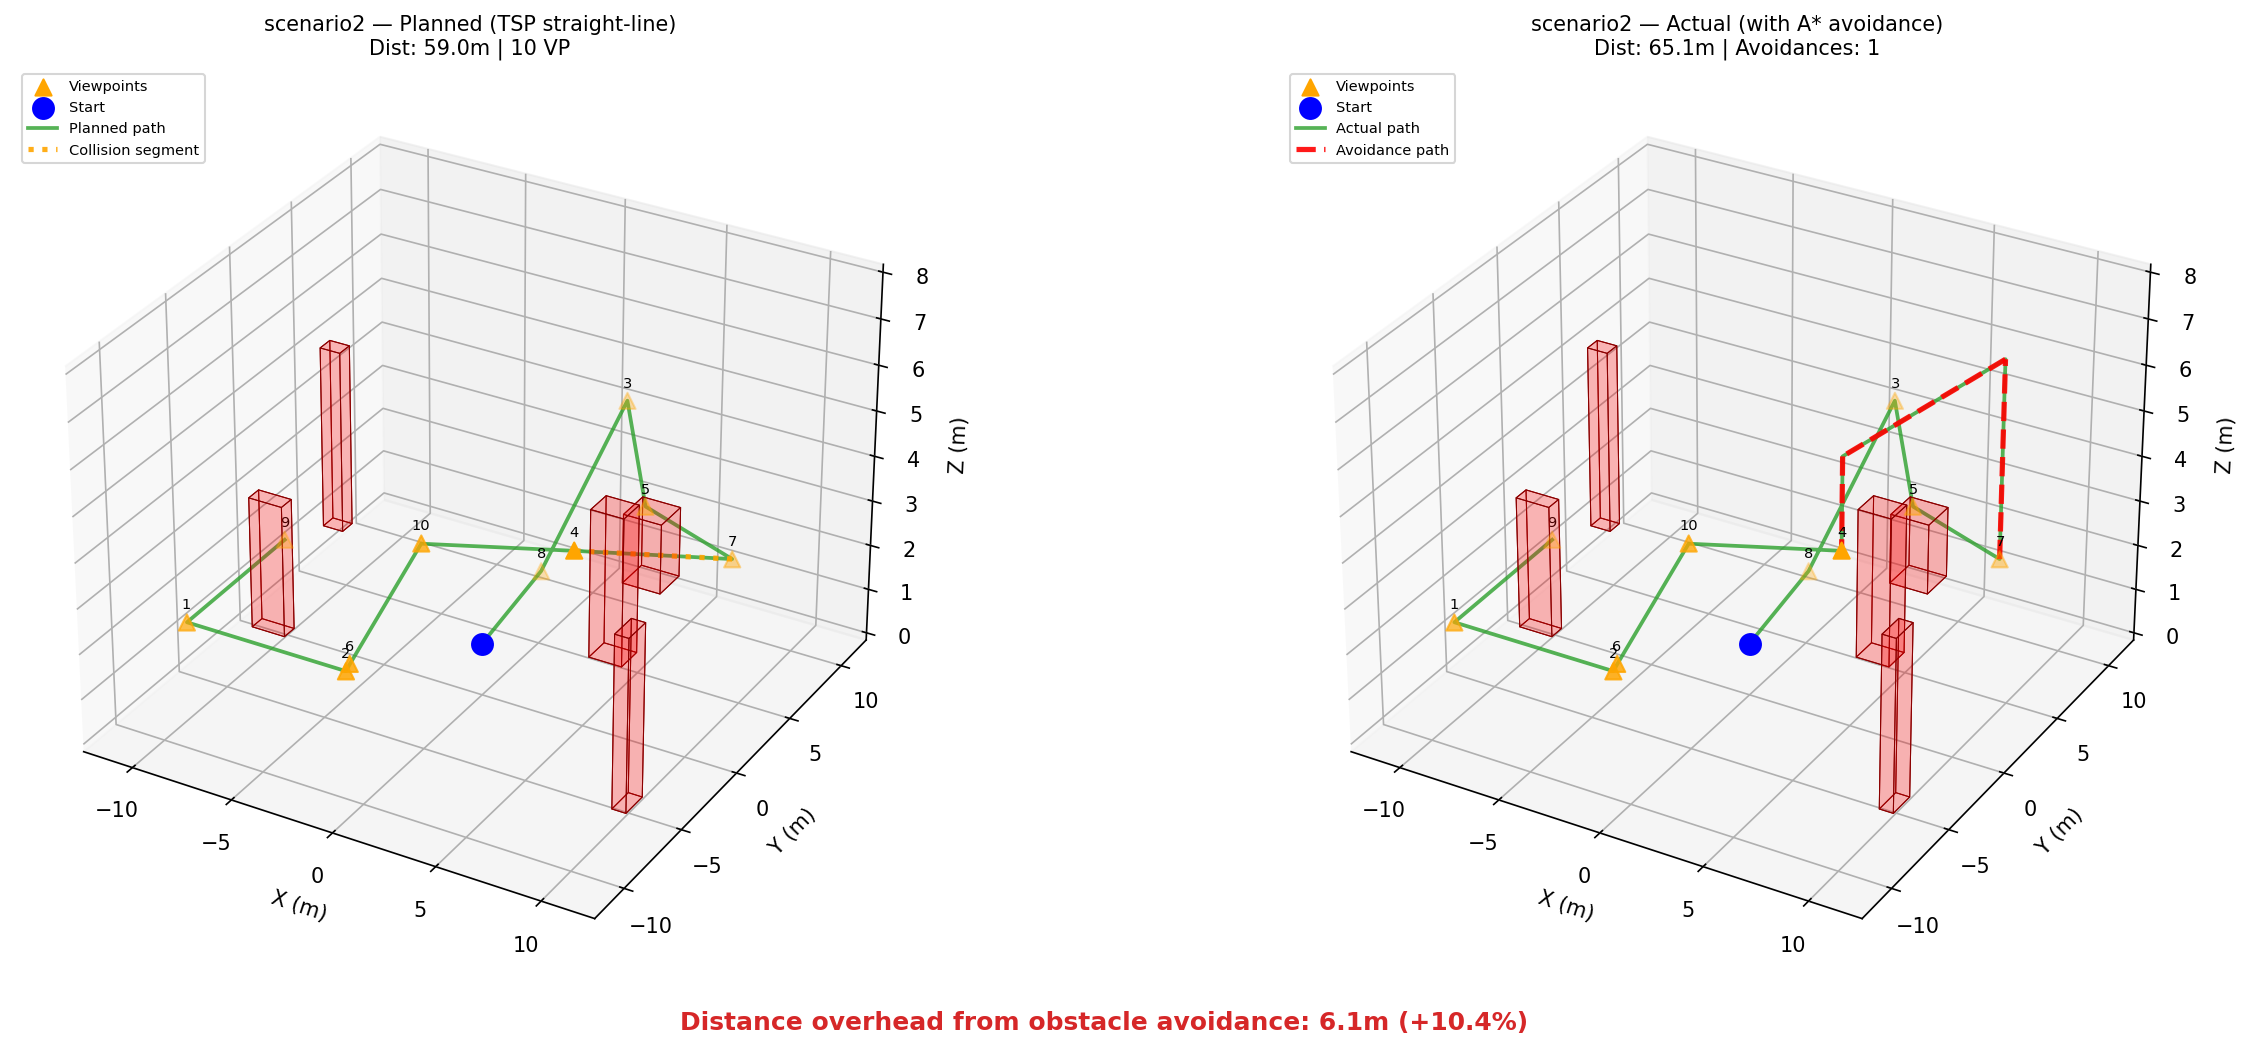
\includegraphics[width=0.48\textwidth]{visualisations/vis_scenario2_planned_vs_actual.png}\\[0.3cm]
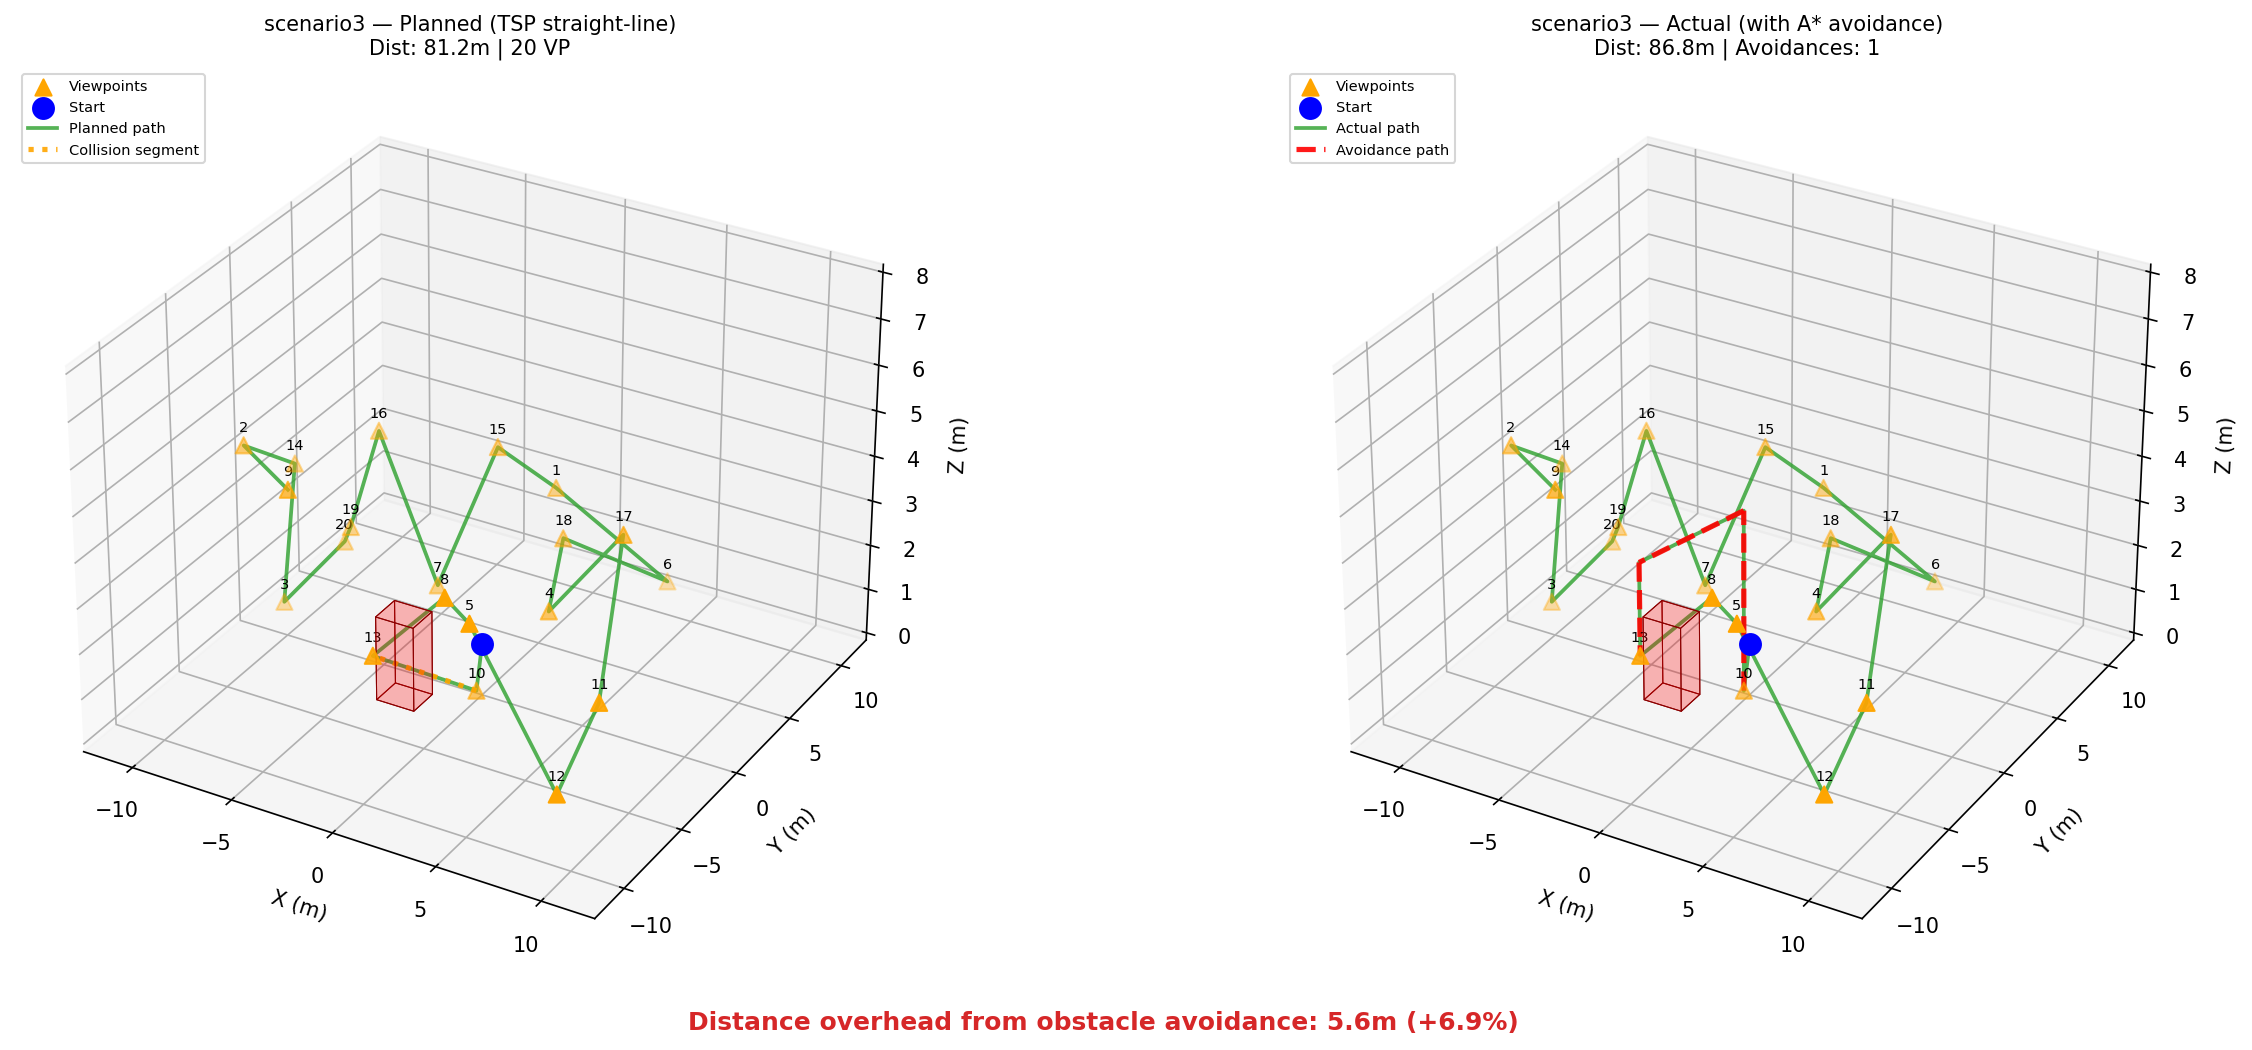
\includegraphics[width=0.48\textwidth]{visualisations/vis_scenario3_planned_vs_actual.png}
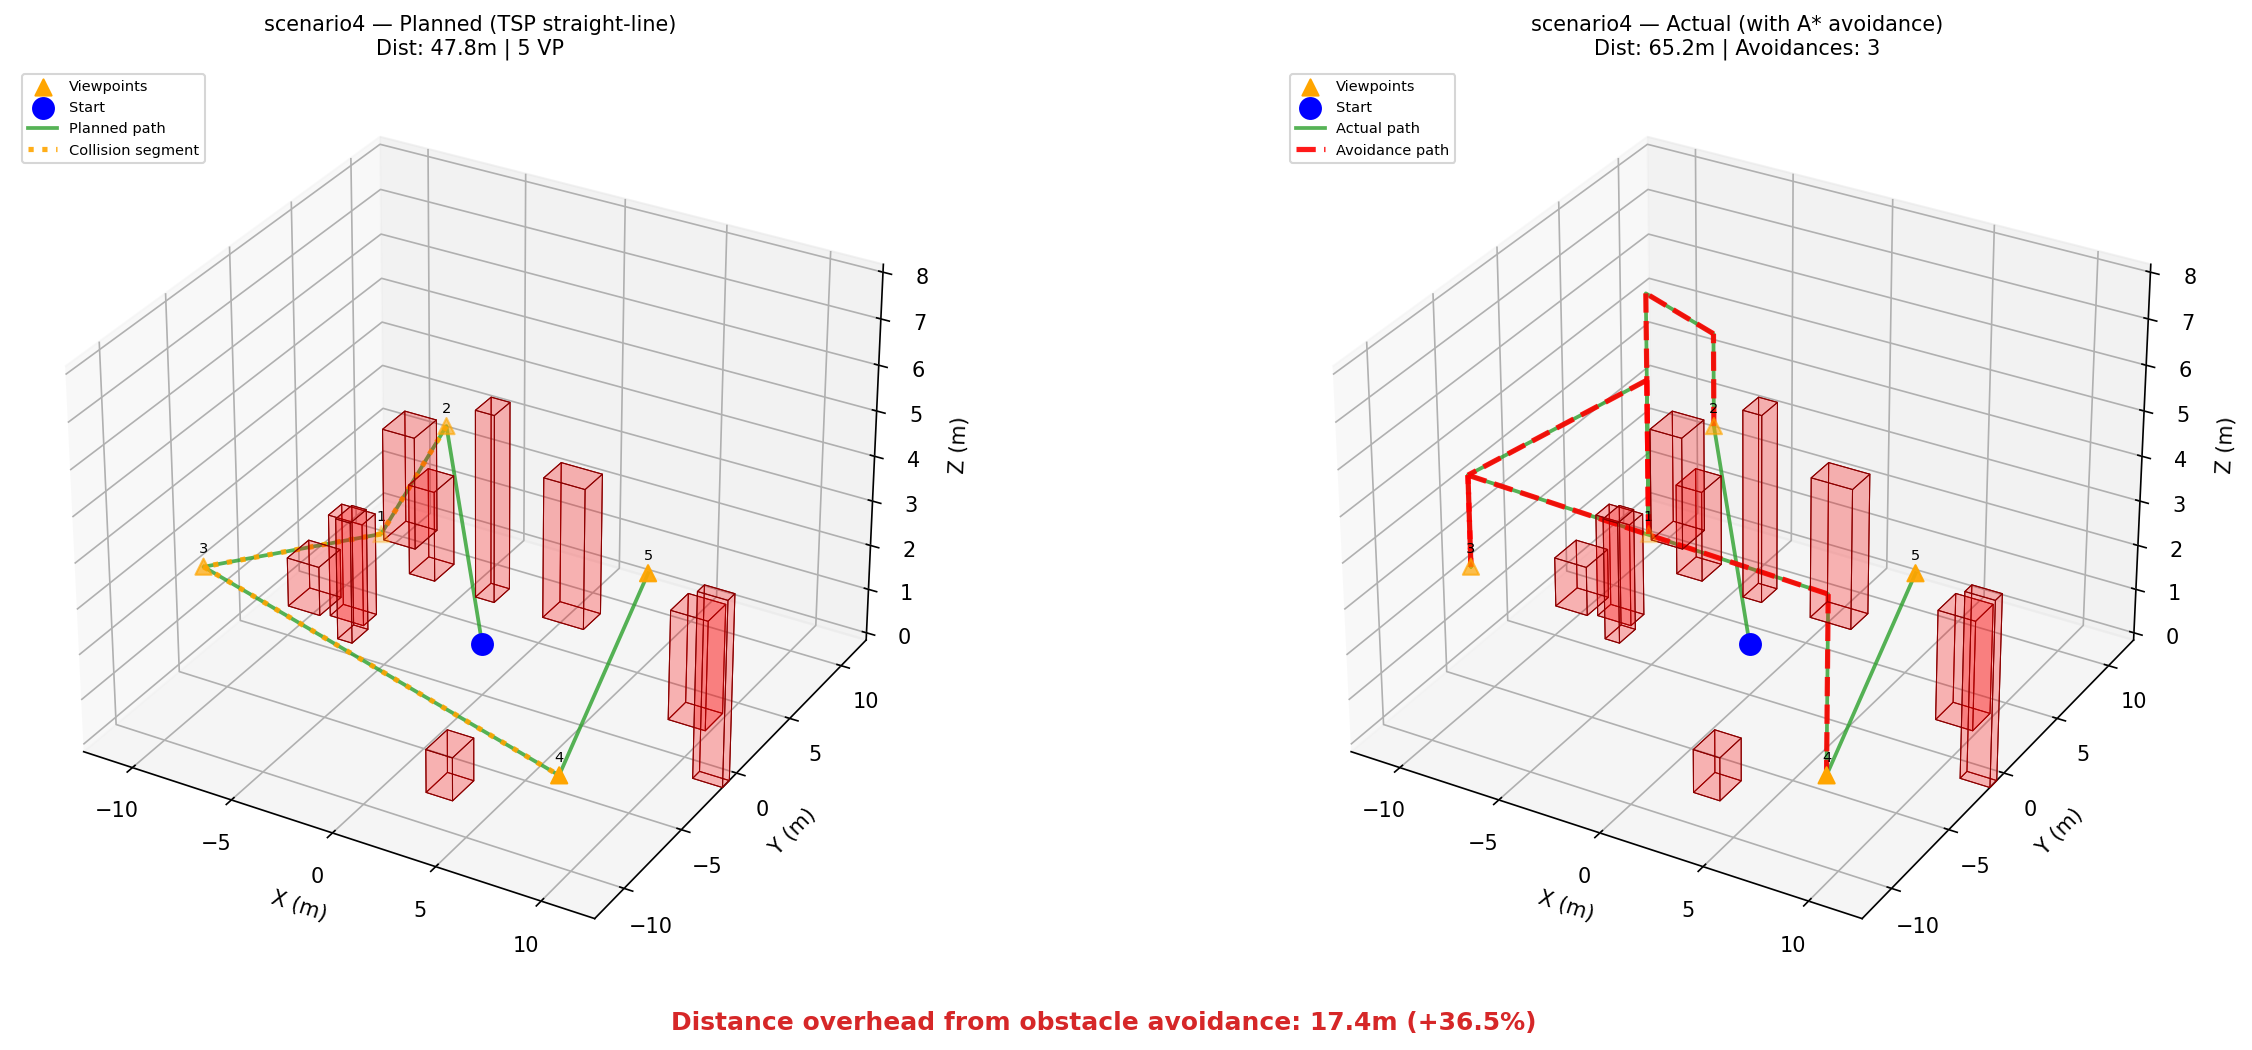
\includegraphics[width=0.48\textwidth]{visualisations/vis_scenario4_planned_vs_actual.png}
\caption{Planned (TSP straight-line, left) vs actual (with A* avoidance, right) flight paths for all four scenarios. Orange dotted lines indicate collision segments; red dashed lines show avoidance paths.}
\label{fig:planned_actual}
\end{figure}

\section{Conclusions}

The combined TSP + A* approach achieves 100\% success across all scenarios while reducing flight time by 45--48\% and distance by 53\% compared to the sequential baseline. The three-tier obstacle avoidance strategy—elevation bypass, A* search, and high-altitude fallback—provides robust collision-free navigation with acceptable distance overhead (6.9--36.5\% depending on obstacle density). The hybrid TSP solver (exact DP for $n \leq 15$, simulated annealing otherwise) scales effectively from 5 to 20 viewpoints. Key engineering decisions include converting yaw angles from radians to degrees, using 1.0m obstacle padding for safety, and employing blocking flight commands to ensure reliable waypoint reaching. Future improvements could incorporate obstacle-aware TSP formulations that jointly optimise visitation order and avoidance paths.

\end{document}
